In \cite{mutolo2025path}, a ``balancing'' heuristic was proposed as a baseline approach to distributing Bell-pairs.  The baseline heuristic distributes Bell pairs among the network using a simple criterion.  Any node $n$ that was eligible for a swap would consider all pairs of nodes $i$,$j$, $i \ne j \ne n$, and if both $Q_{ni}(t), Q_{nj}(t) > Q_{ij}(t) + 1$, then, noting that implementing a swap that completes at time $t + \delta t$ would satisfy $Q_{ni}(t+\delta t) = Q_{ni}(t)-1, Q_{nj}(t+\delta t) = Q_{nj}(t)-1, Q_{ij}(t) = Q_{ij}(t+\delta t) = Q_{ij}(t) + 1$ while satisfying $Q_{ni}(t+\delta t), Q_{nj}(t+ \delta t) \ge Q_{ij}(t + \delta t)$, such a swap would be marked as {\em preferred}, meaning it satisfied the max-min criteria of transferring commodity from entities that initially had more to entities that initially had less, such that after the transfer, those initially with more remained no smaller than those with initially less (i.e., a better balance).  The intuition behind this approach was that by balancing resources throughout the Quantum network, Bell pairs would flow naturally away from points of generation where inventory (Bell pairs) was continually restocked, and toward points of consumption where inventory was continually drained.  Since the node $n$ can only perform a single swap, it must choose from its set of preferred swapping candidates which to perform.  That paper selects the pair $i,j$ for which $Q_{ij}(t)$ is minimal.

Mutolo et al also formulate a linear program that identifies the feasible region for which there exists a swapping process that can satisfy a given allocation of generation and consumption rates.  They do not explicitly speculate on how well this max-min heuristic does at covering the feasible region.  Further, since the swapping graph is fully connected, the paper states that ``Were generation and consumption to both cease, this swapping process would balance Bell pairs in the network such that the minimum count would be maximized, i.e., when no swap candidates are preferrable, a max-min fair allocation has been established, in that no buffer count can be increased without reducing another that was already smaller.''  While not explicitly stated, one might infer that this means that ``balanced'' would mean that the difference between any pair counts would be at most 1 (i.e., there is some integer $N$ for which $Q_{ij} \in \{N,N-1\}$ for all $i,j$.  

We now demonstrate that this inference is wrong by producing a simple counter-example, and use this counterexample to show that the max-min heuristic can fail to meet consumption demands even when there exists a swapping strategy that could do so.
\begin{center}
\begin{figure}[!htb]
\centering
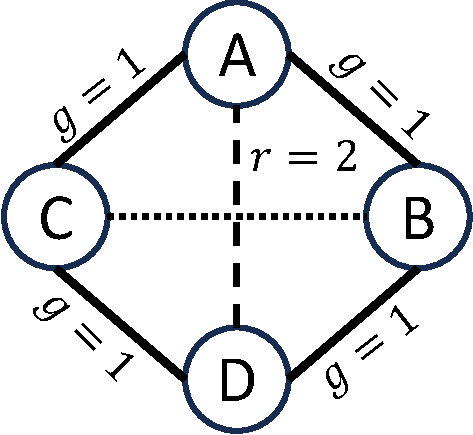
\includegraphics{Fig/BackPressure-MaxMin-CounterExample-crop.pdf}
\caption{A canonical example of a network that has no preferrable swaps.}
\label{fig:maxmin-counterexample}
\end{figure}
\end{center}

Figure \ref{fig:maxmin-counterexample} depicts a small, 4-node fully-connected network where each edge represents the Bell pair count ($Q$) between node pairs, where each count is either $N$ or $m < N$.  Note that according to the aforementioned definition of {\em preferrable}, there is no 3-node combination where a swap is preferrable: The only 3-node combination that could be preferrable is one where there are two edges of size $N$ and a third of size $m$.  If any two are of size $m$, one must be reduced in the swapping process.  Note $m$ can be much smaller than $N$, i.e., it need not be the case that $m$ is anything close to $N-1$.  Note further that even if there were small discrepancies among the edges labeled by $N$ (i.e., each edge's count $N_{AB}, N_{BC}, N_{CA}$ differed slightly and $m_{AD}, m_{BD}, m_{CD}$ differed slightly, but where $N_{ij} \gg m_{kD}$ for all $i,j,k \in \{A,B,C\}$, there would still be no swapping from edges not connected to $D$ to edges connected to $D$.

Now, consider a setting where $N \gg m$ and generation rates are $X \lambda$ along each edge that is labeled by $X \in \{m,N\}$, and consumption rates are $m \lambda + \epsilon$ along every edge.  Note the edges excluding $D$ all generate at rate $N \lambda$ and consume at rate $m \lambda + \epsilon$ such that their queues grow at rate $(N-m) \lambda - \epsilon$.  Furthermore, edges that include $D$ generate at rate $m \lambda$ and consume at rate $m \lambda + \epsilon$, such that they develop a backlog of consumption requests at rate $\epsilon$.  This means that over time, a situation similar to that depicted in Figure \ref{fig:maxmin-counterexample} will ensue where edges not connected to $D$ will grow with large stores of Bell pairs (i.e., $((N-m) \lambda - \epsilon) t$ by time $t$), edges connected to $D$ will have no Bell pairs but an ever-growing (unbounded) queue of unsatisfied consumption requests (of size $\epsilon t$ by time $t$).  Note further that this phenomenon would occur regardless of the strategy used by nodes to select which of a set of preferrable edges gets swapped: there are simply no preferrable edges to choose from!
